% ----------------------------------------------------
% Literature Review
% ----------------------------------------------------
\documentclass[class=report,11pt,crop=false]{standalone}
% Page geometry
\usepackage[a4paper,margin=20mm,top=25mm,bottom=25mm]{geometry}
\usepackage{indentfirst}
% Font choice
\usepackage{lmodern}

% Use IEEE bibliography style
\bibliographystyle{IEEEtran}

% Line spacing
\usepackage{setspace}
\setstretch{1.20}

% Ensure UTF8 encoding
\usepackage[utf8]{inputenc}

% Language standard (not too important)
\usepackage[english]{babel}

% Skip a line in between paragraphs
\usepackage{parskip}

% For the creation of dummy text
\usepackage{blindtext}

% Math
\usepackage{amsmath}

\usepackage{enumitem}


% Header & Footer stuff
\usepackage{fancyhdr}
\pagestyle{fancy}
\fancyhead{}
\fancyhead[R]{\nouppercase{\rightmark}}
\fancyfoot{}
\fancyfoot[C]{\thepage}
\renewcommand{\headrulewidth}{0.0pt}
\renewcommand{\footrulewidth}{0.0pt}
\setlength{\headheight}{13.6pt}

% Epigraphs
\usepackage{epigraph}
\setlength\epigraphrule{0pt}
\setlength{\epigraphwidth}{0.65\textwidth}

% Colour
\usepackage{color}
\usepackage[usenames,dvipsnames]{xcolor}

% Hyperlinks & References
\usepackage{hyperref}
\definecolor{linkColour}{RGB}{77,71,200}%{0,144,208}%
\hypersetup{
    colorlinks=true,
    linkcolor=linkColour,
    filecolor=linkColour,
    urlcolor=linkColour,
    citecolor=linkColour,
}
\urlstyle{same}

% Automatically correct front-side quotes
\usepackage[autostyle=false, style=ukenglish]{csquotes}
\MakeOuterQuote{"}

% Graphics
\usepackage{graphicx}
\graphicspath{{Images/}{../Images/}}
\usepackage{makecell}
\usepackage{transparent}

% SI units
\usepackage{siunitx}

% Microtype goodness
\usepackage{microtype}

% Listings
\usepackage[T1]{fontenc}
\usepackage{listings}
\usepackage[scaled=0.8]{DejaVuSansMono}

% Custom colours for listings
\definecolor{backgroundColour}{RGB}{250,250,250}
\definecolor{commentColour}{RGB}{10, 204, 10}
\definecolor{identifierColour}{RGB}{0, 0, 255}%{196, 19, 66}
\definecolor{stringColour}{RGB}{255, 0, 255}
\definecolor{keywordColour}{RGB}{255,0,0}
\definecolor{lineNumbersColour}{RGB}{127,127,127}
\lstset{
  language=Python,
  captionpos=b,
  aboveskip=10pt,belowskip=10pt,
  backgroundcolor=\color{backgroundColour},
  basicstyle=\ttfamily,%\footnotesize,        % the size of the fonts that are used for the code
  breakatwhitespace=false,         % sets if automatic breaks should only happen at whitespace
  breaklines=true,                 % sets automatic line breaking
  postbreak=\mbox{\textcolor{red}{$\hookrightarrow$}\space},
  commentstyle=\color{commentColour},    % comment style
  identifierstyle=\color{identifierColour},
  stringstyle=\color{stringColour},
   keywordstyle=\color{keywordColour},       % keyword style
  %escapeinside={\%*}{*)},          % if you want to add LaTeX within your code
  extendedchars=true,              % lets you use non-ASCII characters; for 8-bits encodings only, does not work with UTF-8
  frame=single,	                   % adds a frame around the code
  keepspaces=true,                 % keeps spaces in text, useful for keeping indentation of code (possibly needs columns=flexible)
  morekeywords={*,...},            % if you want to add more keywords to the set
  numbers=left,                    % where to put the line-numbers; possible values are (none, left, right)
  numbersep=5pt,                   % how far the line-numbers are from the code
  numberstyle=\tiny\color{lineNumbersColour}, % the style that is used for the line-numbers
  rulecolor=\color{black},         % if not set, the frame-color may be changed on line-breaks within not-black text (e.g. comments (green here))
  showspaces=false,                % show spaces everywhere adding particular underscores; it overrides 'showstringspaces'
  showstringspaces=false,          % underline spaces within strings only
  showtabs=false,                  % show tabs within strings adding particular underscores
  stepnumber=1,                    % the step between two line-numbers. If it's 1, each line will be numbered
  tabsize=2,	                   % sets default tabsize to 2 spaces
  %title=\lstname                   % show the filename of files included with \lstinputlisting; also try caption instead of title
}

% Caption stuff
\usepackage[hypcap=true, justification=centering]{caption}
\usepackage{subcaption}

% Glossary package
% \usepackage[acronym]{glossaries}
\usepackage{glossaries-extra}
\setabbreviationstyle[acronym]{long-short}

% For Proofs & Theorems
\usepackage{amsthm}

% Maths symbols
\usepackage{amssymb}
\usepackage{mathrsfs}
\usepackage{mathtools}

% For algorithms
\usepackage[]{algorithm2e}

% Spacing stuff
\setlength{\abovecaptionskip}{5pt plus 3pt minus 2pt}
\setlength{\belowcaptionskip}{5pt plus 3pt minus 2pt}
\setlength{\textfloatsep}{10pt plus 3pt minus 2pt}
\setlength{\intextsep}{15pt plus 3pt minus 2pt}

% For aligning footnotes at bottom of page, instead of hugging text
\usepackage[bottom]{footmisc}

% Add LoF, Bib, etc. to ToC
\usepackage[nottoc]{tocbibind}

% SI
\usepackage{siunitx}

% For removing some whitespace in Chapter headings etc
\usepackage{etoolbox}
\makeatletter
\patchcmd{\@makechapterhead}{\vspace*{50\p@}}{\vspace*{-10pt}}{}{}%
\patchcmd{\@makeschapterhead}{\vspace*{50\p@}}{\vspace*{-10pt}}{}{}%
\makeatother
\makenoidxglossaries


\newacronym{fm}{FM}{Frequency Modulation}
\newacronym{am}{AM}{Amplitude Modulation}
\newacronym{em}{EM}{electromagnetic}
\newacronym{iq}{IQ}{In-phase and Quadrature}


\newacronym{dft}{DFT}{Discrete Fourier Transform}
\newacronym{idft}{IDFT}{Inverse Discrete Fourier Transform}
\newacronym{fft}{FFT}{Fast Fourier Transform}
\newacronym{ifft}{IFFT}{Inverse Fast Fourier Transform}

\newacronym{df}{DF}{Direction Finding}
\newacronym{rdf}{RDF}{Radio Direction Finding}
\newacronym{AoA}{AoA}{Angle of Arrival}
\newacronym{rf}{RF}{Radio Frequency}
\newacronym{sdr}{SDR}{Software-Defined Radio}
\newacronym{pd}{PD}{Phase-Difference}
\newacronym{vhf}{VHF}{Very High Frequency}
\newacronym{MHz}{MHz}{Megahertz}
\newacronym{db}{dB}{decibel}
\newacronym{dbm}{dBm}{Decibel-milliwatts}
\newacronym{rx}{Rx}{Receiver}
\newacronym{tx}{Tx}{Transmitter}
\newacronym{dsp}{DSP}{Digital Signal Processing}
\newacronym{vor}{VOR}{Very High Frequency Omnidirection Range}
\newacronym{gps}{GPS}{Global Position System}
\newacronym{adf}{ADF}{Automatic Direction Finders}
\newacronym{ndb}{NDB}{Non-Directional Beacon}
\newacronym{sm}{S meter}{Signal Strength Meter}
\newacronym{tdoa}{TDOA}{Time Difference of Arrival}
\newacronym{ham}{HAM}{an informal name for an amateur radio operator}
\newacronym{wbfm}{WBFM}{Wideband Frequency Modulation}
\newacronym{if}{IF}{Intermediate Frequency}
\newacronym{lp}{LP}{Low Pass}
\newacronym{API}{API}{Application Programming Interface}
\newacronym{fpga}{FPGA}{Field-Programmable Gate Array}
\newacronym{bw}{BW}{Bandwidth}
\newacronym{adc}{ADC}{Analog-to-digital converter}
\newacronym{tv}{Tv}{Television}
\newacronym{ai}{AI}{Artificial Intelligence}
\newacronym{lo}{LO}{Local Oscillator}
\newacronym{icasa}{ICASA}{Independent Communications Authority of South Africa}
\newacronym{usb}{USB}{Universal-serial Buss}
\newacronym{os}{OS}{Operating System}
\newacronym{mimo}{MIMO}{Mutliple input, Multiple output}
\newacronym{vna}{VNA}{Vector Network Analyser}
\newacronym{mse}{MSE}{Mean Squared Error}
\newacronym{SNR}{SNR}{Signal-to-Noise Ratio}

\begin{document}
\ifstandalone
\tableofcontents
\fi
% ----------------------------------------------------
\chapter{Literature Review and Background \label{ch:literature}}
\epigraph{``All seats provide equal viewing of the universe.''}
    {\emph{---Museum Guide, Hayden Planetarium}}
\vspace{0.5cm}
% ----------------------------------------------------
This chapter aims to establish the surrounding ideas and previous works of the project. By looking into the broader sphere of \gls{sdr} as well as \gls{rdf}, a clearer path may be laid.

A rudimentary \gls{df} system can be constructed quickly and without knowledge of the internal workings. To implement a more adept \gls{df} system in the digital domain requires a deeper understanding of the underlying processes and theories of both \gls{em} waves and \gls{dsp}. A fundamental understanding of the \gls{fft} and antenna theory would additionally yield a more finely tuned system.
Therefore, the literature discussed here hopes to give a general backdrop to the reader and provide insight into the theories used in the project, including motivation for the project and the existing work surrounding it.

This chapter begins by \textbf{\emph{briefly}} examining \gls{em} waves and radio history which form the fundamental underlying concepts of a \gls{sdr}. These independent concepts have a complicated and interesting history, as well as a complex theoretical foundation, much too intricate to fully cover in this report. Nevertheless, important concepts are analysed which sets the stage for the next discussion of \gls{sdr} itself: covering both the history and workings of such devices. Then, with an understanding of how radio and \gls{sdr} work, an analysis of \gls{df} is presented, covering theoretical understanding and the different algorithms that are used in typical \gls{df} systems, with a brief departure from \gls{sdr} to discuss wildlife telemetry methods. The penultimate section of this chapter makes mention of similar work and the current devices that are of a comparable nature to this project. The chapter is wrapped up by a short literature critique, outlining the value of this project. 

%---------------------------------------------------------------------------------------------------%
                                    % Electromagnetic waves
%---------------------------------------------------------------------------------------------------%
\section{Traditional Radio}
Various communication forms have evolved over time, from spoken word to modern satellites. It goes without saying that communication systems are limited by the media over which they are transmitted. Underpinning the idea of \gls{sdr} explored in the next section is the desire to manipulate and use the \gls{em} spectrum, of which radio is a portion of this spectrum. 
%---------------------------------
% Brief History
%---------------------------------
\subsection{Brief History}
Radio enjoys a complex and interesting history, and like many scientific breakthroughs, attributing the development of radio to a single individual would be rather disingenuous. 

There remains much literature debate about who is credited for the invention of the radio \cite{radio-history}. Whether it be Nikolai Tesla or Guglielmo Marconi, the first wireless telegraphy patent was awarded to Marconi in 1896. 

Before they were able to perform their experiments, however, a Scottish mathematical physicist published seminal work. In 1865, James Maxwell published "A Dynamical Theory of the Electromagnetic Field" \cite{maxwell1865viii}, in which the famous Maxwell's equations were first demonstrated. Within the collection of 20 equations, Maxwell predicted that \gls{em} waves travelling through free space would travel at the speed of light \cite{maxwell2}. 

Three decades later, Heinrich Hertz was able to verify these equations \cite{hertz1893electromagnetic}, and although "electromagnetic radiation" is the formal scientific term today, what Heinrich Hertz demonstrated with his simple spark transmitter experiment lay the foundation for \gls{rf} development. 

The generally accepted history is that radio developed as a signalling and audio communication technique using \gls{em} radiation, and was first used as a "wireless telegraph" where regular telegraphy lines were impractical. It then developed into the ability to simultaneously broadcast messages to multiple locations, first using the dots-and-dashes associated with Morse Code, and later to full audio \cite{radio-development}.

In the late 1800s, at the time of Radio's development, it was generally assumed that \gls{em} waves required a medium to propagate, and this medium was called "ether".
%---------------------------------
% Propagation
%---------------------------------
\subsection{Propagation}
When discussing \gls{em} waves, the basic theoretical understanding of how these waves propagate is necessary. Firstly Radio waves can propagate from transmitter to receiver in four ways: 
\begin{itemize}
    \setlength{\itemsep}{0pt}
    \item ground waves
    \item sky waves
    \item free space waves
    \item open field waves
\end{itemize}

While radio waves are transmitted in accordance with classical electromagnetic theory, they are still subjected to reflection, refraction, and scattering effects \cite{radio-propagation}.

These waves are oscillating, electric and magnetic fields, with components in various directions and relative phases between components. 

Prehaps Marconi's most significant discovery with regards to \gls{em} waves was that of the "groundwave" for radio signals \cite{radio-history}. Marconi discovered that by adding a ground connection to a transmitter, the range of transmission was greatly increased. Today, we understand this as the  "earthing" of the transmitter antenna, which results in radio signals using the ground as a waveguide and following the earth's plane. Signals are thus spread out in only two dimensions, unlike a free-space transmission, which disperses into three dimensions.

While the full derivation of the wave equation is not presented in this report, as there is substantial literature presented on this topic, the equations of the wave motion are given \cite{radio-waves}:
\begin{equation}
    \Delta^2 E = \epsilon_0 \mu_0 \frac{\delta^2 E}{\delta^2 t}
\end{equation}
\begin{equation}
    \frac{1}{\sqrt{\epsilon_0 \mu_0}} = 3 \times 10^ 8 = c
\end{equation}
%---------------------------------
% Traditional super het 
%---------------------------------
\subsection{Traditional Superheterodyne}
Before we are able to understand the inner workings of a \gls{sdr}, we must first look at how traditional radios implement the same processing demands in hardware (Figure \ref{fig:traditonal-superhet}). In order to receive high-frequency \gls{rf} signals, early radios would mix the incoming \gls{rf} signal with a \gls{lo} to produce the \gls{if}. During mixing with the \gls{lo}, both sum and difference frequencies are created, and the \gls{if} filter filters out the sum frequency, leaving only the difference to be demodulated. This allows traditional radios to demodulate high-frequency \gls{rf} waves. 

\begin{figure}[h]
    \centering
    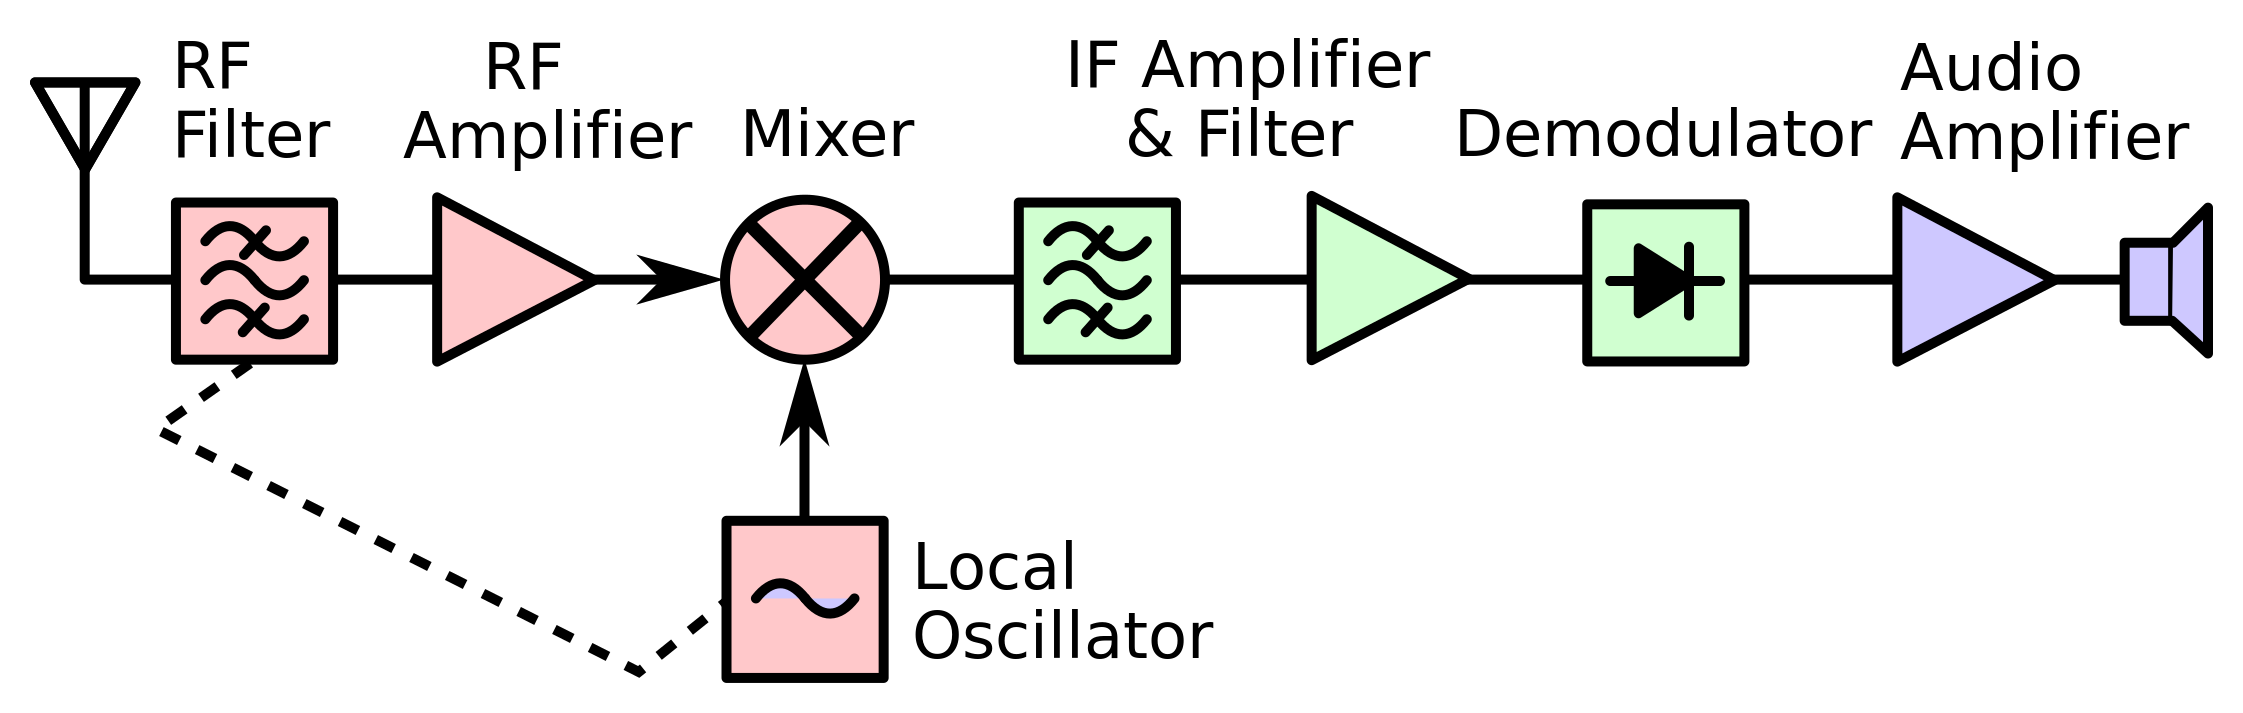
\includegraphics[width=0.8\textwidth]{Images/diagrams/Superheterodyne_receiver_block_diagram.png}
    \caption{A block diagram of the traditional Superheterodyne Architecture \cite{superhet}}
    \label{fig:traditonal-superhet}
\end{figure}
%---------------------------------------------------------------------------------------------------%
                                    % Software Defined Radio
%---------------------------------------------------------------------------------------------------%
\section{Software Defined Radio}

%---------------------------------
% Brief History
%---------------------------------
\subsection{Brief History}
Much like radio itself, \gls{sdr}, has a convoluted yet interesting history. With the rapid growth in \gls{rf} design corresponding to the evolution of transistors, \gls{sdr} was developed from a stream of successive discoveries.

Joe Mitola first used the phase \emph{software radio} in 1991 \cite{sdr-modern-approach}, to refer to a reprogrammable/reconfigurable radio class. Dr. Jeffery Reed furthered this definition by defining a \gls{sdr} as any radio that can be substantially defined in software, and whose physical behaviour is able to be altered through changes to that software \cite{sdr-modern-approach}.

With advancements in low-cost electronics and \gls{dsp}, we now have the ability to manipulate shorter-wavelength portions of the \gls{em} spectrum as a function of frequency. The ability to do this is due to the architecture of modern \gls{sdr} platforms.

%---------------------------------
% Architecture
%---------------------------------
\subsection{Architecture}
Nychis et.al \cite{sdr-arch} classifies \gls{sdr} into two main architectures:
\begin{itemize}
    \item Host-PHY Architecture (Figure \ref{fig:hostphy}) is the most common architecture, which enables redesign and development of the entire transceiver system in software. This system provides the most flexibility because of its design. The drawback of such a system is the processing and communication delays associated with the architecture. 
    \item NIC-PHY Architecture is implemented by using a \gls{fpga} and a \gls{dsp} front-end. By being located in close proximity to the radio hardware, and by utilizing specialized parallel hardware processing, this architecture improves the communication delays associated with Host-PHY. This does, however, translate to a system that is time-consuming and difficult to design, and subsequently more complex. 
\end{itemize}

Ideally, the digital sampling would occur immediately following the reception of the signal from the antenna, however, this approach is not practical for \gls{rf} signals. \gls{sdr} architectures thus begin with the traditional superheterodyne approach and then implements the \gls{if} Amplifier, Filters and Demodulators within the digital domain with software as illustrated in figure \ref{fig:sdr-arch}.
\begin{figure}[h]
    \centering
    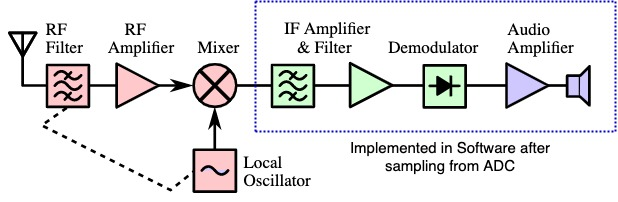
\includegraphics[width=0.8\textwidth]{Images/diagrams/superhet_software.jpg}
    \caption{Replacement of the traditional Superheterodyne architecture in software \cite{superhet}}
    \label{fig:sdr-arch}
\end{figure}

Since the most commonly used \gls{sdr} architecture is the Host-Phy (Figure \ref{fig:hostphy}), this discussion is based on it. The system can be broken into two main components, namely the \gls{sdr} platform and the Host Computer. 

\begin{figure}[h]
    \centering
    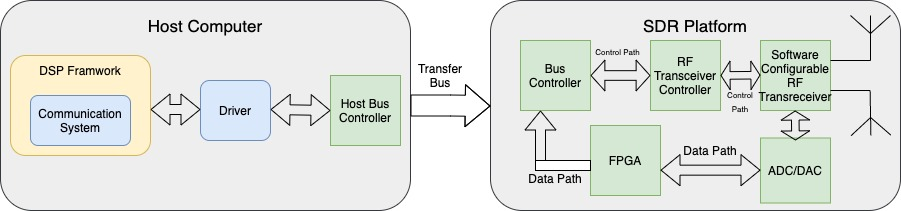
\includegraphics[width=0.8\textwidth]{Images/diagrams/SDR.jpg}
    \caption{A block diagram of a typical Host-PHY Software Defined Radio architecture adapted from \cite{sdr-arch}}
    \label{fig:hostphy}
\end{figure}

The \gls{sdr} platform itself is the hardware that provides access to \gls{rf} signals and naturally is flexible. In transceiver systems, \gls{rf} signals are both transmitted (\gls{tx}) and received (\gls{rx}) by the platform. These analogue signals are converted by the \gls{adc} to digital samples and then transferred to the host computer. 

The host computer is a general-purpose computer, and the control system as well as the communication system. The host computer runs the software to process the digital signals from the samples received by the \gls{sdr} platform. It is also used during initialisation to configure the \gls{sdr}.

%---------------------------------
% Interfacing
%---------------------------------
\subsection{Interfacing}
Interfacing with an \gls{sdr} is the first hurdle to accomplish in developing any \gls{sdr} project, and often times this is not a simple process as drivers and operating systems are constantly updated. While by no means a complete description, Figure \ref{fig:limeSDR-interfacing-soapy}, provides an overview of the various software packages available to use when interfacing with a \gls{sdr} in particular the LimeSDR. 
\begin{figure}[h]
    \centering
    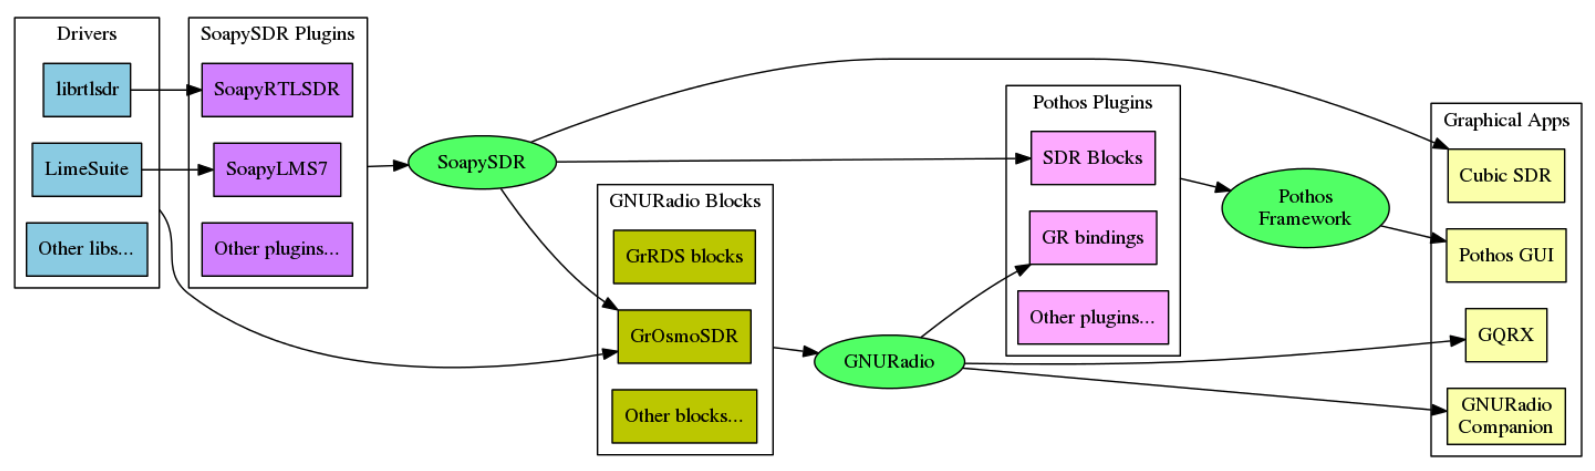
\includegraphics[width=0.8\textwidth]{Images/diagrams/interfacing_LimeSDR.png}
    \caption{The various software packages used for interfacing devices to the LimeSuite and SoapySDR \cite{limesuite-soapy}}
    \label{fig:limeSDR-interfacing-soapy}
\end{figure}

\subsubsection{GNU-Radio}
GNU Radio is an open-source \gls{dsp} framework, which has seen rapid evolution thanks to a large, active community. GNU-Radio provides a graphical interface for designing signal processing chains. With an easy to use framework and extensive support for most \gls{sdr} platforms, as well as a large library, this is the most common \gls{sdr} programming software.

GNU-Radio is capable of streaming large amounts of data between parallel computational nodes in real-tine, which is controlled by the built in scheduler. This scheduler schedules the execution of blocks within a flow graph. From a designer point of view, these blocks can be viewed to be executing concurrently.

\subsubsection{SoapSDR API}
Of particular importance to this project is the SoapySDR \gls{API}. One can think of this as the glue layer that binds the LimeSDR's driver to other \gls{sdr} applications.
Additionally, SoapySDR comes with \textsc{Python} bindings to connect, control, test and develop with the LimeSDR. These bindings provide almost complete control of the board, and while \textsc{Python} is not the language of choice for performance, allow for simpler development. 

\begin{figure}
    \centering
    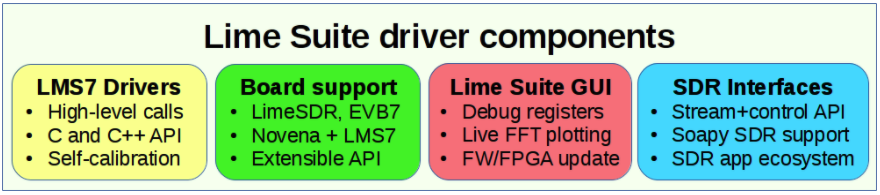
\includegraphics[width=0.8\textwidth]{Images/diagrams/LimeSuite.png}
    \caption{Description of various driver components associated with LimeSuite \cite{limesuite}}
    \label{fig:LimeSuite}
\end{figure}
%---------------------------------------------------------------------------------------------------%
                                    % Direction Finding
%---------------------------------------------------------------------------------------------------%
\section{Direction Finding}
The history of \gls{df} naturally is interlaced with that of radio. While the invention of the radio changed the way we were able to communicate, the introduction of the transistor radio revolutionised communication yet again. Portable and compact radios give rise to exciting and new possibilities in \gls{rf} engineering. This section covers a brief history, as well as the commonly used algorithms in \gls{df} systems.

%---------------------------------
% Brief History 
%---------------------------------
\subsection{Brief History}
Heinrich Hertz carried out the earliest experiments in \gls{rdf} in 1888, discovering that the  directionality of an open loop of wire used as an antenna, pointed in different directions would change the gain of said antenna \cite{hertz-expeirments}. By the early 1900s, \gls{df} methods had evolved and in World War I, both sides were able to use \gls{df} to locate enemy positions on the ground. It was at this time that the essential principles of direction-finding were established, well before even commercial radio use in the 1920s \cite{df-history}

The first known commercial use for \gls{df} was the transmission of Morse code from a \gls{ndb} at a low frequency (known as \gls{adf}). Pilots would note the Morse code in pre-flight briefings and then fly in the direction of the transmission frequency. This aviation method lead to the invention of both \gls{vor} and \gls{gps}.

Come World War II, an \gls{rdf} operator, while tuned to a frequency of interest, manually turned the loop of the antenna and used a \gls{sm} to determine the direction of the null (weakest signal) \cite{df-history}.

Fast forward to today, and there are multiple ways to discover the location of a transmitted signal, mainly due to the abilities of \gls{sdr}. The majority of \gls{df} systems fall within two categories, namely trilateration and triangulation. With multiple antennas, the most commonly used system is trilateration, illustrated on the left of Figure \ref{fig:Tri vs Tri }. By measuring the time difference of the signal between each receiver, trilateration is able to measure the distances from different reference points. This technique  produces the pseudo-range, and the location can be acquired by observing the common area. Contrasting, triangulation (illustrated right, Figure \ref{fig:Tri vs Tri }) produces a location by computing angles relative to different reference points. This produces bearings, and where these bearings intersect is the theoretical location. 

\begin{figure}[h]
    \centering
    \captionsetup{type=figure}
    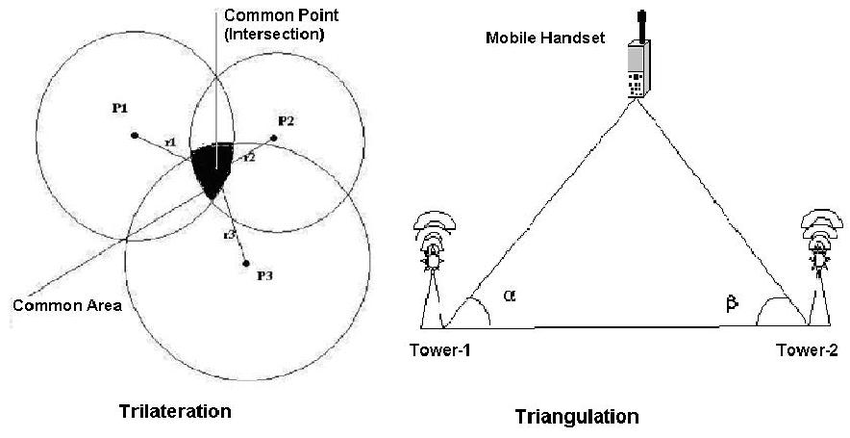
\includegraphics[width=0.8\textwidth]{../Images/diagrams/tri_vs_tri.png}
    \caption{Graphical explanation of trilateration vs triangulation         \cite{triangulation-vs-trilateration} }
    
    \label{fig:Tri vs Tri }
\end{figure}

In order to reduce the complexity of the system, reduce receiver locations and cost, the exact location of a transmitter can be acquired with the use of a single receiver in a single location, using multiple \gls{rx} antenna. 

%---------------------------------
% Algorithms for df 
%---------------------------------
\subsection{Algorithms for Radio Direction Finding}
Since the direction of a radio signal can be estimated using either the amplitude or the phase (in fact both would work) of the signal, many \gls{df} algorithms have been developed, each with different advantages and disadvantages. This section discusses some of the more common algorithms and uses this as a base for the selection of the algorithm to be used for this project. 

\subsubsection{Watson-Watt}
A fairly complicated, but widely uses method is the Adcock/Watson-Watt method. These methods are theoretically similar and will be discussed as such for the remainder of this chapter, with the only difference being in the antenna arrangement. The Adcock method uses an antenna array consisting of a pair of antennas (monopole or dipole) that exploits the vector difference of each received signal at the individual antenna to produce only one output for each pair of antennas \cite{ww-df}. If the pairs of antennae are co-located but perpendicularly oriented, we note the pairs as N-S (North-South) and E-W (East-West). At the receiver, taking the
\begin{equation}
    \arctan{\frac{(N-S)}{(E-W)}}
    \label{ww-equation}
\end{equation}
will produce the bearing angle. 

Conversely, the Watson-Watt method used the same two antenna pairs to perform an amplitude comparison of the received signals with the addition of an omnidirectional, vertically polarized electric dipole. This resolves the ambiguities arising from the Adcock method \cite{ww-patent}.

Looking at Figure \ref{fig:ww-diagram}, the output of each antenna pair can be mathematically represented as \cite{ww-diagram}:
\begin{equation}
    x(t) = V_a \cos(\varphi) \cos(\omega t)
\end{equation}
\begin{equation}
    y(t) = V_a \sin(\varphi) \cos(\omega t)
\end{equation}

Where $V_a$ is the maximum antenna output in Volts.

The \gls{rf} signal is then converted to a \gls{if} by the receiver. The signals are demodulated by mixing each signal with a reference signal $R(t)$. After a \gls{lp} filter removes high-frequency components, the resultant outputs are then given by:

\begin{equation}
    R(t) = V_r \cos(\omega t)
\end{equation}
\begin{equation}
    X = V_0 \cos(\varphi)
\end{equation}
\begin{equation}
    Y = V_0 \sin(\varphi) 
\end{equation}

Finally, remembering equation \ref{ww-equation}, the bearing angle produced by the Watson-Watt method can be calculated as:
\begin{equation}
    \theta_c = \arctan(\frac{Y}{X})
\end{equation}

$\theta_c$ is only unique if the reference is derived from a signal which has a phase independent of the signal bearing. A further explanation into methods for producing this is not required in this report, as the basic workings of the method do not include this. Suffice to say, this popular method is sensitive to frequency changes and narrow-band assumptions \cite{df-issues}, with the accuracy being highly reliant on the post-processing of the information. As such this method will not be used for this project. 

\begin{figure}[h]
    \centering
    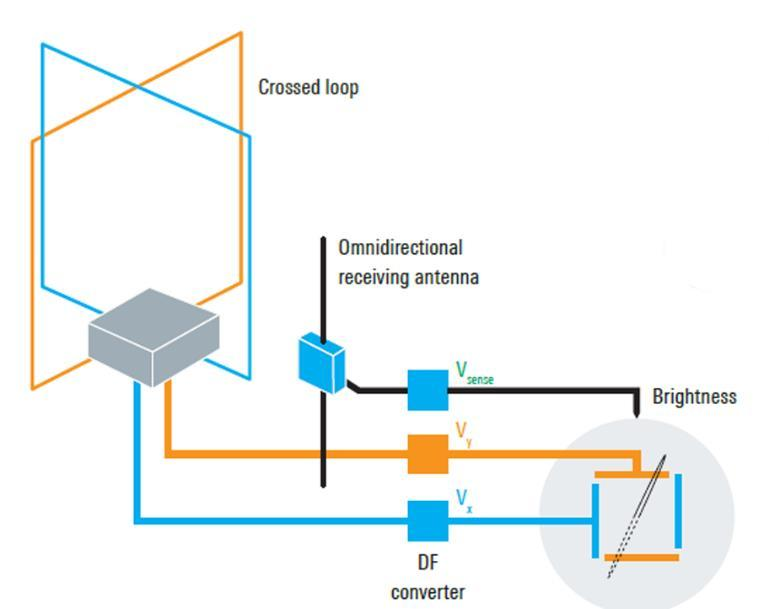
\includegraphics[width=0.6\textwidth]{Images/diagrams/ww-geom.jpg}
    \caption{Working diagram of the Watson-Watt Method \cite{ww-diagram}}
    \label{fig:ww-diagram}
\end{figure}
    
\subsubsection{Pseudo-Doppler}
A Doppler \gls{rdf} system is based on relative motion between the transmitter and a receiver \cite{pd-thesis}. This motion can be produced by physically rotating the antenna themselves (True Doppler) or by electronically switching between antenna in an array (Pseudo Doppler) \cite{pd-thesis}. This method of \gls{rdf} was first used by amateur HAM \footnote{The term HAM is \gls{ham} but due to the prevalence of the term in literature will be used as a common noun in this report.} radio operators and has since found tracking in wildlife telemetry applications \cite{pd-wildlife}, however, the accuracy of this method is still not fully-fledged.

The performance of this technology is based on both the algorithm implemented and the size and number of antenna elements within the array. To avoid multi-path phase ambiguity, the radius size of the pseudo-Doppler antenna array must be less than half of the wavelength of the signal received.

Looking at Figure \ref{fig:pd geometry}, let's assume the antenna are switched, in a clockwise fashion, giving (A-B-C-D) \cite{pd-thesis}. This switching would produce the Doppler shift, detecting the approach or withdrawal of the signal. A signal originating from direction A, would produce a zero shift at position A, a minimum shift at position B, and the maximum shift at position D due to the approaching position of the signal. Note that the phase \emph{jumps} are due to electronic switching. 

\begin{figure}[h]\centering
    \subfloat[Stationary Antenna Arrangement in a Pseudo Doppler array]{\label{a}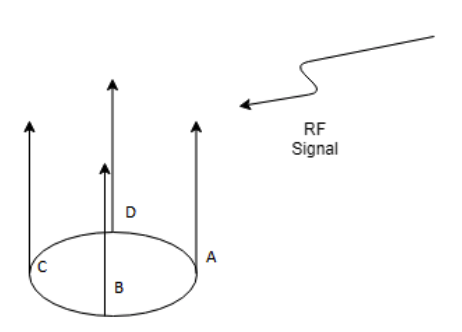
\includegraphics[width=.4\linewidth]{Images/diagrams/pd-1.png}}
    \subfloat[Output pulses received due to rotation of array]{\label{b}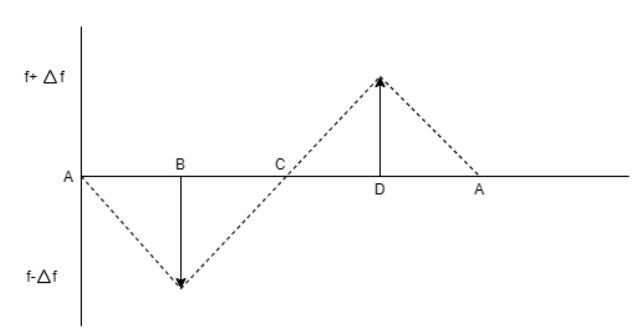
\includegraphics[width=.4\linewidth]{Images/diagrams/pd-2.png}} 
    \caption{Pseudo Doppler array arrangement and resulting Doppler Shifts \cite{pd-thesis}}
    \label{fig:pd geometry}
\end{figure}

The phase created by each antenna during shifting is given by \cite{pd-thesis}:
\begin{equation}
    \frac{2 \pi r}{\lambda} \cos{(\frac{2 \pi i}{N} - \theta)}
\end{equation}

Assuming that there are $N_a$ monopole antenna in the circular array of radius ’r’, and the receiver switches from i$th$ antenna to the $(i + 1)th$ antenna.

Leading to the time-varying phase shift \cite{pd-thesis}:
\begin{equation}
    \Theta_s(t) = \frac{2 \pi r}{\lambda} \cos{(\frac{2\pi}{N_a} \sum_{n=1}^{\infty} (u(t-nT_s) - \theta))}
\end{equation}

where $u(t)$ is the unit step function and $\theta$ is the \gls{AoA}.
This method, while suited to the project, has two major drawbacks. Firstly, because the "movement" in pseudo-Doppler is electronically controlled by switching steps, the resulting signal contains phase \emph{jumps}. This additionally produces a signal with considerable numbers of sidebands. \cite{pd-sidebands}  The switching system furthermore introduces electronic noise. 
Secondly,  pseudo Doppler \gls{rdf} must have a constant signal \emph{within its bandwidth} to produce sensible results. This means that this technique cannot handle multiple signals, which for wildlife telemetry makes it obsolete. Additionally, for testing on \gls{wbfm} stations, this would prove difficult, and any other wide digital signals with noise is simply impractical.

Note that the rate at which switching occurs is critical to the performance of the system, and while this is theoretically realisable in software,  \cite{pd-gnu}, this method is not fully developed and hardware implementations are costly.



\subsubsection{\gls{tdoa}}
Time Difference of Arrival is arguably the second most commonly used location finding technique. The versatility of this method lies in the fact that only the time of the signal being received and the speed with which that signal travellers matters in the calculation. Once the target signal has been received at at least two reference points, the difference in arrival time can be used to calculate each distance to the target and the individual reference points using the equation \cite{tdoa-formula}:
\begin{equation}
    \Delta d = c * \Delta t  
    \label{eq:distance}
\end{equation}

Where \emph{c} is the speed of light in a vacuum and $\Delta t $ is the arrival time difference relative to each reference point. Dealing with the location of the reference points in a two-dimensional space yields \cite{tdao-2d}:
\begin{equation}
    \Delta d = \sqrt{(x_2 - x)^2 + (y_2 - y) ^2} - \sqrt{(x_1 - x)^2 + (y_1 - y)^2}
\end{equation}

where $(x_1, y_1)$ and $(x_2, y_2)$ are the known coordinates of the reference points. From this we can see that using \gls{tdoa} from at least three transmitters would be needed to produce the exact location of the receiver, being the intersection of the hyperboloids. Solving the system of hyperbola equations is performed through either linear regression or by the Taylor series expansion \cite{tdao-2d}.

\begin{figure}[h]\centering
    \subfloat[Example Setup]{\label{a}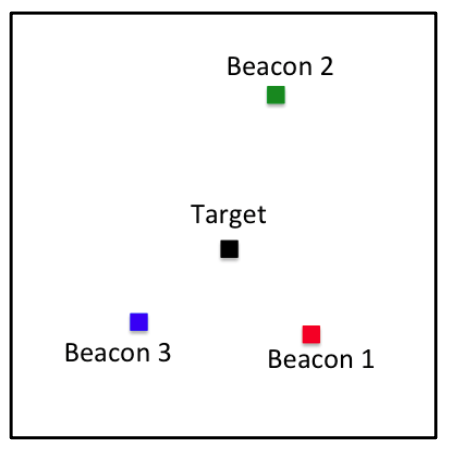
\includegraphics[width=.3\linewidth]{Images/diagrams/tdoa_1.png}}\hfill
    \subfloat[Possible locations relative to beacon 2]{\label{b}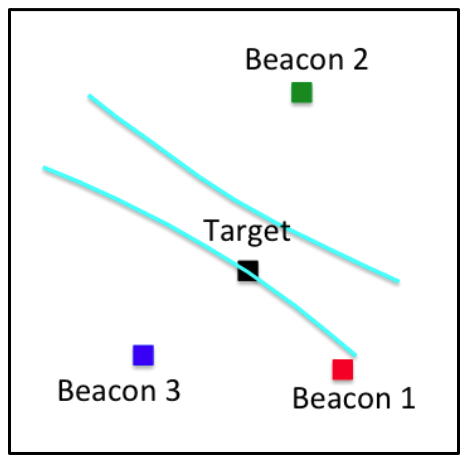
\includegraphics[width=.3\linewidth]{Images/diagrams/tdoa_2.png}}\hfill 
    \subfloat[All possible locations]{\label{c}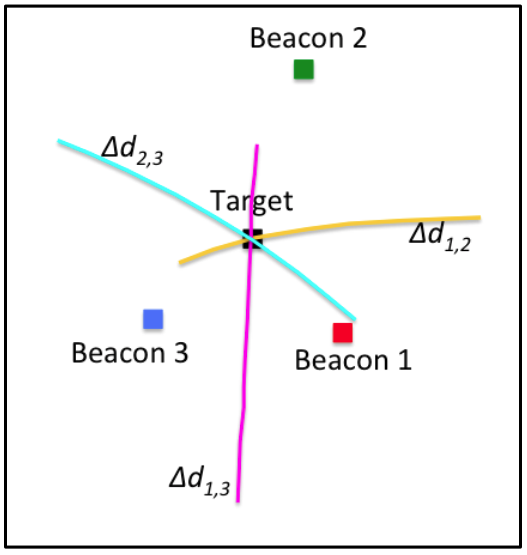
\includegraphics[width=.28\linewidth]{Images/diagrams/tdoa_3.png}}
    \caption{Geometrical representation of calculations steps for Time Difference of Arrival \cite{tdoa-calculation}}
    \label{tdao geometry}
\end{figure}

%\cite{tdoa} what is this? 

The time resolution required for an accurate \gls{tdoa} system is impractical for the nature of this project. To give and example: Sampling at a rate of 10 MHz would yield a time resolution of:
\begin{equation*}
    time = \frac{1}{frequency} = \frac{1}{10 \si{MHz}} = 0.1 \si{\micro . s}
\end{equation*}

And using equation \ref{eq:distance} to correspond the time resolution to a spatial resolution error of:
\begin{equation*}
    d = 3 \times 10^8 \si{\meter . s^{-1}} * 0.1 \si{\micro . s} = 30 \si{\meter} 
\end{equation*}

Noting, that one cannot simply increase the sampling rate, as if we increase the sample rate beyond the bandwidth of the signal, the variations between successive data samples are increasingly related to noise rather than to variations in the signal \cite{crfs_2021}.

\subsubsection{Phase Interferometry}

Since this is the principle on which the project is built, further detail into the derivation of the algorithms and \gls{dsp} theory will be performed in Chapter \ref{ch:meth}. A brief overview of the literature and discussion on advantages and disadvantages will however still follow.

Phase Interferometry differs from the \gls{tdoa} approach in that while the method still relies on the time delay of arrival of signals between multiple antennae, the measurement of the difference in received signal phase is performed, and not the relative time difference \cite{Phase-comparison}. This method is thus accurate over short distances, as the relative time is not needed within the calculation itself. At each (a minimum of 3 if one wishes to remove the ambiguity of angles) \gls{rx} antenna, the phase of the received signal is measured as the imaginary component of the signal, which is usually represented as complex \gls{iq} data \footnote{This important concept, which underpins modern \gls{sdr} will further be analysed in Chapter \ref{ch:meth}}. However, for now, we can note by processing \gls{iq} data, we reduce the complexity of determining the frequency and phase of a signal \cite{smith}. The general equation of a real-valued sin wave is given by:
\begin{equation}
    x(t) = A \sin(2 \pi f t + \phi)
    \label{eq:general}
\end{equation}
Using trigonometric identities, we can rewrite equation \ref{eq:general} as:
\begin{equation}
    x(t) = A\sin(\phi)\cos(2\pi f t) + A\cos(\phi)\sin(2\pi f t)
\end{equation}
\begin{equation}
    x(t) = A_1\cos(2\pi f t) + A_2\sin(2\pi f t)
    \label{eq:IQ-general}
\end{equation}
Where $A_1 = A\sin(\phi)$ and $A_2 = A\sin(\phi)$ \cite{phase-diff-calc}. These two sinusoidal components are representative of the \gls{iq} form. The $\sin$ (in-phase) component, and the $\cos$ (quadrature) component:

\begin{equation}
    I = A_2 \sin(2 \pi f t) 
    \label{eq:I}
\end{equation}
\begin{equation}
    Q = A_2 \cos(2 \pi f t)
    \label{eq:Q}
\end{equation}

To convert \gls{iq} components from polar coordinates to the Cartesian plane is shown in Figure \ref{fig:IQ}. With \gls{iq} representative of the signal, we are now able to use equation \ref{eq:iq} to calculate the instantaneous phase.

\begin{figure}[h]
    \centering
    \captionsetup{type=figure}
    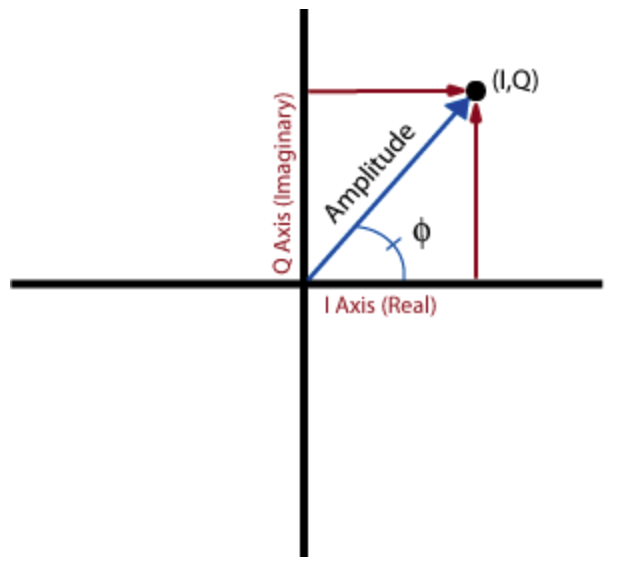
\includegraphics[width=0.4\textwidth]{Images/diagrams/iq.png}
    \caption{Polar and I-Q coordinates, where $\phi$ is the phase, I is the real component of the wave and Q is the imaginary component.}
    \label{fig:IQ}
\end{figure}

\begin{equation}
    \theta = \arctan(Q/I)
    \label{eq:iq}
\end{equation}


Noting that while Phase comparison is perhaps the most accurate technique for providing a bearing angle, it is also the most demanding technique from a control perspective \cite{phase-comparison-issues}. This method both relies upon tight calibration and synchronisation. Since a slight difference between channels can lead to negligible phase measurements, the system requires that each channel is time-aligned. With respect to synchronisation, when this system is implemented with a digital receiver, it is critical that the receiver is able to synchronise the channels. 

This method additionally has a trade-off between the sampling rate, frequency of interest and the \gls{bw} being analysed \cite{Phase-comparison}. When the distance between antenna is of a similar scale ($ \frac{\lambda}{2}$) to the wavelength of the received signal, the phase difference is significant enough to be able to measure efficiently \cite{phase-comparison-issues}.

Figure \ref{fig:phase_interfer} shows the setup of a two-antenna phase interferometry system, with the associated trigonometry used to produce the phase difference. Leading to the equation of interest for this system \cite{phase-diff-calc}: 
\begin{equation}
    \theta = \arcsin(\frac{\lambda \Delta \phi}{2 \pi s} ) 
    \label{eq:pd-theta}
\end{equation}

Where $\lambda$ is the wavelength of the received \gls{rf} signal, $\Delta \phi$ is the difference in phase between each antenna,  restricted between $0$ and $2\pi$, and $s$ is the horizontal distance between the \gls{rx} antenna \cite{phase-diff-calc}. 

\begin{figure}[h]
    \centering
    \captionsetup{type=figure}
    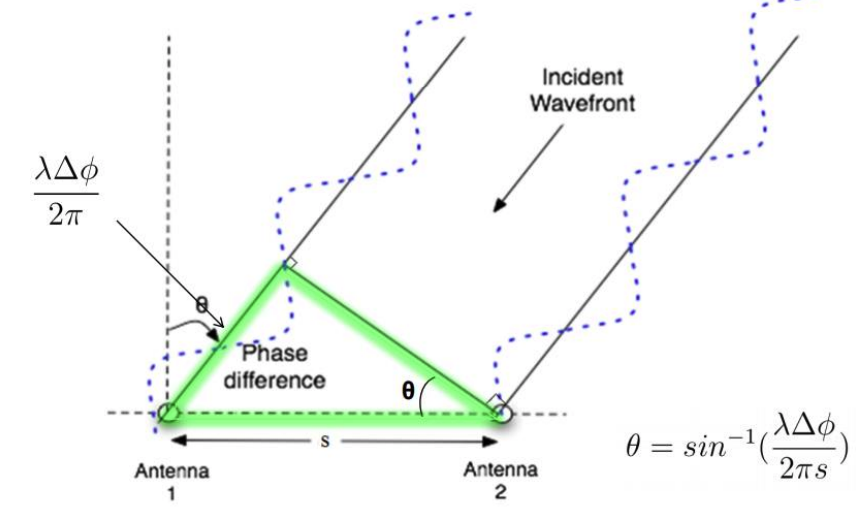
\includegraphics[width=0.7\textwidth]{Images/diagrams/phase_interferometry.png}
    \caption{Geometrical representation of Phase Interferometry usage}
    \label{fig:phase_interfer}
\end{figure}

To conclude \gls{df} algorithms, one could implement any of the above-mentioned systems, or in fact a combination of the different technologies. However, common issues occur in each, namely reflections, interferences, hardware limitations and modulation errors \cite{df-issues}. 
%---------------------------------
% Animal Tracking
%---------------------------------
\subsection{Current Methods of Animal Tracking}
Wildlife scientists have used radio telemetry to track  animal movement and behaviour for many years. 
The basic ideology for radio-tracking animals is to allow scientists the ability to gain further insight into animal behaviour, migration patterns, the health of individuals and more recently, provide protection in the case of rhino poaching. While this report does not need to detail the need for advancements in radio-tracking from the protection of wildlife, and by extension, natural diversity globally, this point is made. 

In literature, the first known use of animal tracking was by the famous ornithologist, John James Audubon \cite{james-banding}. John conducted the first 'bird banding' experiment, by tying strings to the legs of birds and observing birds that returned to the same nesting site the following year.  

Since then there exist many methods for tracking currently used, with three being more prevalent than the others. \gls{gps} tracking, satellite tracking and \gls{vhf} tracking methods all have advantages and disadvantages. The following discussion will relate to the most common method, \gls{vhf} tracking. 

\gls{vhf} telemetry is defined by a transmitter attached to an animal and a receiver. The receiver  is used by researchers to capture the signal transmitted which in turn is captured by a hand-held directional antenna (usually a yagi). The direction of the signal at its strongest is used to locate the animal in the field. This is the most common telemetry method and has been in use since the mid-1960s \cite{wild-life-telem}. The exact location of the transmitter can then be determined if the transmission signal is acquired from three or more locations, which enables the triangulation of the animal of interest. 

However, radio-tracking as a system can be implemented through a wide variety of additional methods. Simply put, all that is needed to perform radio-tracking is the acquisition of a signal transmitted by a device attached to an animal, by a \gls{rx} antenna attached to a receiver. This is the proposed idea of the project: that by receiving the transmitted signal on one device by two or more antennas, the need for triangulation is eliminated. By processing the data captured by each \gls{rx} antenna, the phase of said signal can be extracted and thus with knowledge of the distances between antennas, allow the system to provide a bearing angle pointing in the direction of the transmission source.


%---------------------------------------------------------------------------------------------------%
                                % Available Technologies
%---------------------------------------------------------------------------------------------------%
\section{Current Available Technologies}

At this stage, it is important to note technologies currently readily available for \gls{df} use.
The first note of a similar project, and of inspiration to this project, was previously implemented by Sam Whiting and Todd Moon at GRCon 17 (GNU Radio Conference 2017) \cite{gnu-con17}. Their project was implemented on older RTL-SDR models, using coherent clock synchronisation. Their project still needed cross-correlation to further synchronise the received samples. The project aimed to locate a handheld transmitter and was implemented on an Android phone.

Additionally there exist two professional consumer projects for \emph{plug-and-play} \gls{df}.
The first being the DD007 direction diner device from Rode and Schwarz \cite{DD007}. This portable device is capable of exporting \gls{iq} data for external analysing and has a working range of 20MHz up to 6GHz and a display bandwidth of 10MHz. There are optional extras to be purchased alongside the device, but an immediate drawback to the device is that the captured signal must have a length of at least 10\si{m}s.

The second, arguably best, professional device is the KerberosSDR. This 4-channel coherent \gls{sdr}, is specifically built for direction finding applications \cite{kerberos}. As far as \emph{plug-and-play} options for devices go, this would be near perfect. Bar the 24MHz to 1.7GHz operating range, this open-source programmable device based off of the RTL-SDR is well suited to this project's application. However, due to the experimental nature of this project and budget constraints, it was not feasible to obtain it. The device is based off R820T2 and RTL2832U chips and has demo software available for most native Linux distributions. 


%---------------------------------------------------------------------------------------------------%
                                % Lit Critique
%---------------------------------------------------------------------------------------------------%
\section{Literature Critique}
While this chapter makes it clear that there are many \gls{df} papers available in literature, and cited in this paper, there exist very few experiments using \gls{pd} calculations based off a \gls{sdr} to fundamentally prove that \gls{df} is possible using this technique. Furthermore, there is no comprehensive discussion of the interface between an \gls{sdr} and host-computer, with insight into the \gls{dsp} algorithms and processes needed to produce a \gls{df} system. 

In this chapter, much has already been discussed about the theoretical underpinnings of each associated technology. By providing a top-down approach, first noting the important theoretical understanding of \gls{em} waves and the radio itself, then providing a thorough understanding of \gls{sdr} technologies, this paper aims to fill the gap in literature.

Although in the case of \gls{df}, papers and books have demonstrated successful receiver architectures, outlined signal extraction techniques, and considered error analysis thoroughly, precious little information exists with the underlying goal of using these systems in wildlife telemetry. Wildlife telemetry itself has been around for decades, and the systems critiqued and tested, yet still remains rather under-developed considering the advances in modern \gls{sdr} and signal processing systems.



% ----------------------------------------------------
\ifstandalone
\bibliography{Bibliography/References}
\printnoidxglossary[type=\acronymtype,nonumberlist]
\fi
\end{document}
% ----------------------------------------------------